\documentclass[11pt]{article}
\usepackage[spanish]{babel}

\usepackage{amssymb}
\usepackage{enumerate}
\usepackage{geometry}
\usepackage{mathtools}
\usepackage{multicol}
\usepackage{soul}

\usepackage{graphicx}
	\graphicspath{ {assets/} }


%%%%%%%%%%%%%%%%%%%%%%%%%%%%%%%%%%
%%%%%%%%%%%%%%%%%%%%%%%%%%%%%   %%
%%        Datos Trabajo     %%  %%
%%%%%%%%%%%%%%%%%%%%%%%%%%%%%%%%%%

\newcommand{\titulo}[0]{Evidencia de Aprendizaje . Matrices Gauss-Jordan}
\newcommand{\materia}[0]{\'Algebra Lineal}
\newcommand{\grupo}[0]{BI-BALI-2002-B1-012}
\newcommand{\unidad}[0]{Unidad 2}


%%%%%%%%%%%%%%%%%%%%%%%%%%%%%%%%%%
%%%%%%%%%%%%%%%%%%%%%%%%%%%%%%%%%%

\usepackage[pdftex,
            pdfauthor={bench},
            pdftitle={\titulo},
            pdfsubject={\materia},
            pdfkeywords={\grupo, \unidad, UnADM},
            pdfproducer={Latex with hyperref, or other system},
            pdfcreator={pdflatex, or other tool}]{hyperref}
%%%%%%%%%%%%%%%%%%%%%%%%%%%%%%%%%%
%%%%%%%%%%%%%%%%%%%%%%%%%%%%%%%%%%

\title{
	
\includegraphics{../../../assets/logo-unadm} \\
	\ \\ Benjam\'in Rivera \\
	\bf{\titulo}\\\ \\}

\author{
	Universidad Abierta y a Distancia de México \\
	TSU en Biotecnolog\'ia \\
	\textit{Materia:} \materia \\
	\textit{Grupo:} \grupo \\
	\textit{Unidad:} \unidad \\
	\\
	\textit{Matricula:} ES202105994 }

\date{\textit{Fecha de entrega:} \today}


%%%%%%%%%%%%%%%%%%%%%%%%%%%%%
%%        Documento         %%
%%%%%%%%%%%%%%%%%%%%%%%%%%%%%%%
\begin{document}
\maketitle\newpage

%%%%%%%%%%%%%%%%%%%%%%%%%%%%%%%%
%%          Actividad          %%
%%%%%%%%%%%%%%%%%%%%%%%%%%%%%%%%%%
	\par Resolver en un documento los siguientes sistemas de ecuaciones por el \textbf{Método de Gauss.Jordan} y explica paso a paso. , para hacer seguiremos la siguiente lista de pasos:
	\begin{enumerate}
		\item Normalizaremos el sistema
		\item Representaremos el sistema como matriz ampliada
		\item La manipularemos para obtener una matriz identidad del lado izquierdo 
		\item Leeremos $x_1, x_2 \text{ y } x_3$
	\end{enumerate}
	
	durante el ejercicio usaremos $M_n$ para referirnos a la fila $n$ de la matriz $M$.

\begin{multicols}{2}
	\begin{enumerate}[\bf{Sistema} 1]

		\item 
			\ \\$\begin{matrix}
				2x + 7y + 6z = 48 \\
				4x + 5y + 9z = 24 \\
				3x +  y – 2z = 14 \\
			\end{matrix}$

			\par La matriz extendida resultante de este sistema es
			
			$$\begin{pmatrix}
				2 & 7 & 6 & 48 \\
				4 & 5 & 9 & 24 \\
				3 & 1 & -2 & 14 \\
			\end{pmatrix}$$
			
			ponemos el valor unitario en la primera fila mediante $M_1 = M_1 / 2$, de donde obtenemos
			
			$$\begin{pmatrix}
				1 & \frac{7}{2} & 3 & 24 \\
				4 & 5 & 9 & 24 \\
				3 & 1 & -2 & 14 \\
			\end{pmatrix}$$
			
			y ahora, mediante $M_2 = M_2 - 4M_1$ y $M_3 = M_3 - 3M_1$, rellenamos de ceros la primer columna

			$$\begin{pmatrix}
				1 & \frac{7}{2} & 3 & 24 \\
				0 & -9& -3 &-72 \\
				0 &-\frac{19}{2} &-11&-58 \\
			\end{pmatrix}$$
			
			seguimos con $M_2 = M_2 / -9$ de donde queda
			
			$$\left(\begin{array}{rrrr}
				1 & \frac{7}{2} & 3 & 24 \\
				0 & 1 & \frac{1}{3} & 8 \\
				0 & -\frac{19}{2} & -11 & -58
			\end{array}\right)$$
			
			y luego llenamos con ceros el resto de la columna
			$$\left(\begin{array}{rrrr}
				1 & 0 & \frac{11}{6} & -4 \\
				0 & 1 & \frac{1}{3} & 8 \\
				0 & 0 & -\frac{47}{6} & 18
			\end{array}\right)$$
			
			y repetimos los pasos anteriores, cmabiando los coeficientes, con la ultima fila y columna, para que al final nos quede que
			
			$$\left(\begin{array}{rrrr}
				1 & 0 & 0 & \frac{10}{47} \\
				0 & 1 & 0 & \frac{412}{47} \\
				0 & 0 & 1 & -\frac{108}{47}
			\end{array}\right)$$
			
			de donde obtenemos que		
			\begin{eqnarray*}
				x &=& \frac{10}{47} \\
				y &=& \frac{412}{47} \\
				z &=&-\frac{108}{47}
			\end{eqnarray*}			


		\item
			\ \\ $\begin{matrix}
				x + 12y + 3z = 19 \\
				4 +  5y + 6z = 24 \\
				3 +  7y + 2z = 4
			\end{matrix}$

			\par Priemro pasamos la matriz a su forma normal, de esto queda
			$$\begin{matrix}
				1x + 12y + 3z = 19 \\
				0x +  5y + 6z = 20 \\
				0x +  7y + 2z = 1
			\end{matrix}$$
			
			y su matriz extendida es			
			$$\left(\begin{array}{rrrr}
				1 & 12 & 3 & 19 \\
				0 & 5 & 6 & 20 \\
				0 & 7 & 2 & 1
			\end{array}\right)$$
			
			despues de normalizar proceder\'iamos a modificar la primer columna, pero en este caso ya esta lista, por lo que continuamos con la segunda columna. Primero $M_2 = M_2/5$ para obtener la unidad y luego con $M_1 = M_1 - 12 M_2$ y $M_3 = M_3 - 7 M_2$ limpiaremos para quedarnos con los ceros, de esto queda que 
			$$\left(\begin{array}{rrrr}
				1 & 0 & -\frac{57}{5} & -29 \\
				0 & 1 & \frac{6}{5} & 4 \\
				0 & 0 & -\frac{32}{5} & -27
			\end{array}\right)$$
			
			para la ultima columna empezamos por $M_3 = M_3/(-32/5)$ y luego solo restamos este multiplicado por las veces del coeficiente restante, para que al final nos quede
			$$\left(\begin{array}{rrrr}
				1 & 0 & 0 & \frac{611}{32} \\
				0 & 1 & 0 & -\frac{17}{16} \\
				0 & 0 & 1 & \frac{135}{32}
			\end{array}\right)$$
			
			de esto podemos obtener los valores de la ecuaci\'on, los cuales son
			\begin{eqnarray*}
				x &=& \frac{611}{32} \\
				y &=&-\frac{ 17}{16} \\
				z &=& \frac{135}{32}
			\end{eqnarray*}	

		\item
			\ \\ $\begin{matrix}
				x - 2y + 4z =  7 \\
				4 + 2y - 8z = 10 \\
				2 + 5y + 7z = 23
			\end{matrix}$
			
			\par Primero normalizamos el sistema, de manera que quede		
			$$\begin{matrix}
				1x - 2y + 4z =  7 \\
				0x + 2y - 8z =  6 \\
				0x + 5y + 7z = 21
			\end{matrix}$$
			
			de este sistema obtenemos la siguiente matriz extendida
			$$\left(\begin{array}{rrrr}
				1 & -2 & 4 & 7 \\
				0 & 2 & -8 & 6 \\
				0 & 5 & 7 & 21
			\end{array}\right)$$

			de manera similar al ejercicio anterior, la matriz ya tiene la primer columna lista, por lo que pasamos directamente a trabajar sobre la segunda columna. Comenzamos con $M_2 = M_2/2$ para obtener la unidad y luego con $M_1 = M_1 + 2 M_2$ y $M_3 = M_3 - 5 M_2$ dejaremos la segunda columna tambien lista, de esto queda que
			$$\left(\begin{array}{rrrr}
				1 & 0 & -4 & 13 \\
				0 & 1 & -4 & 3 \\
				0 & 0 & 27 & 6
			\end{array}\right)$$ 
			
			y seguimos el mismo procedimiento con la ultima columna, donde $M_3 = M_3/27$ y se resta la ultima con las otras multiplicada por el coeficiente a eliminar, de donde resulta que
			$$\left(\begin{array}{rrrr}
				1 & 0 & 0 & \frac{125}{9} \\
				0 & 1 & 0 & \frac{35}{9} \\
				0 & 0 & 1 & \frac{2}{9}
			\end{array}\right)$$ 
			
			al final podemos obtener los siguientes resultados
			\begin{eqnarray*}
				x &=& \frac{125}{9} \\
				y &=& \frac{ 35}{9} \\
				z &=& \frac{  2}{9}
			\end{eqnarray*}	

	\end{enumerate}
\end{multicols}




	\subsection*{Comprobaci\'on}
	\par Para corroborar los resutlados se uso el \textit{CAS} 
\footnote{Sistema Algebraico Computacional, por sus siglas en ingles} 
	\href{https://www.sagemath.org/}{SageMath}, que utiliza como interfaz el lenguaje de programaci\'on \href{https://www.python.org/}{Python} y la \textit{UI} jupyter. El archivo html resultante del notebook generado se puede consultar \href{https://github.com/BenchHPZ/UnADM-Biotecnologia/blob/master/B1-1/AL/Actividades/BALI_U2_EA_BERC.ipynb}{aqu\'i}.
	
	\begin{figure}[h]
		\centering
		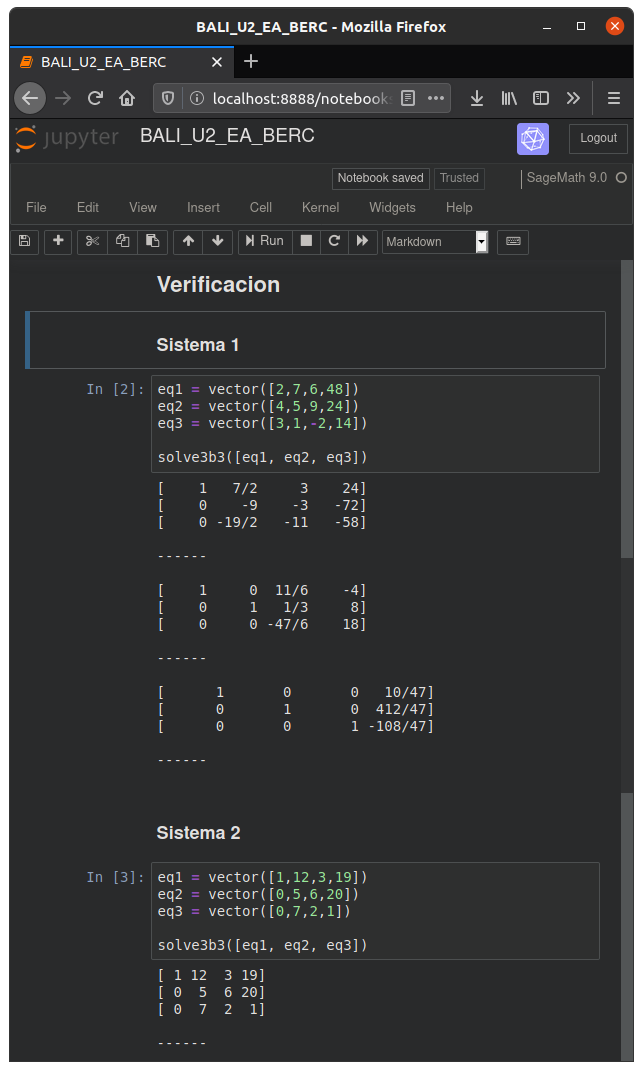
\includegraphics[width=0.32\textwidth]{BALI-U2-EA-1.png}
		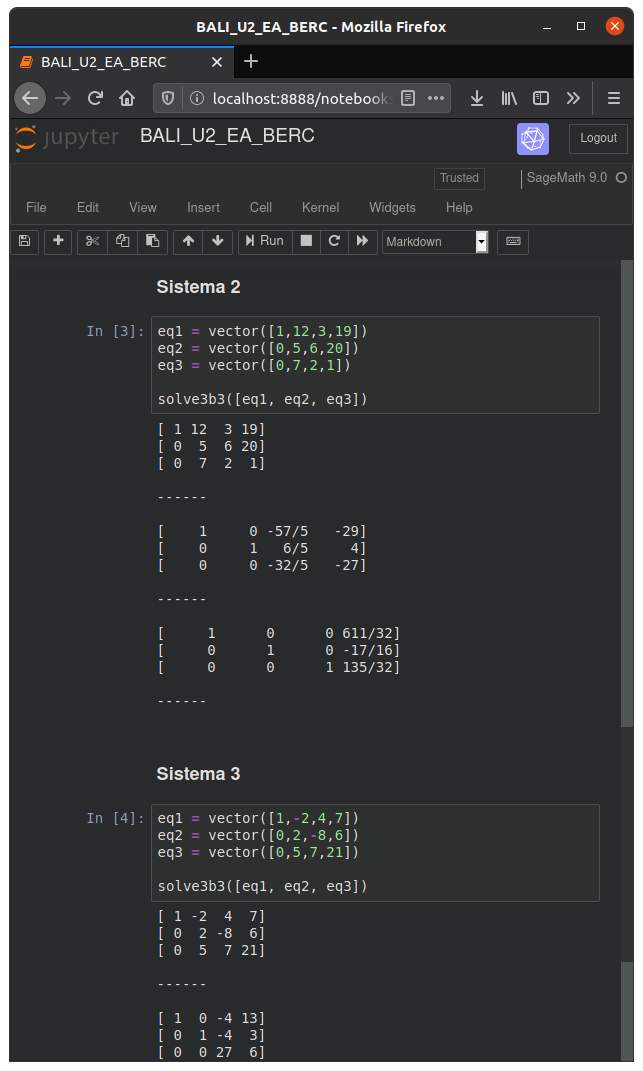
\includegraphics[width=0.32\textwidth]{BALI-U2-EA-2.png}
		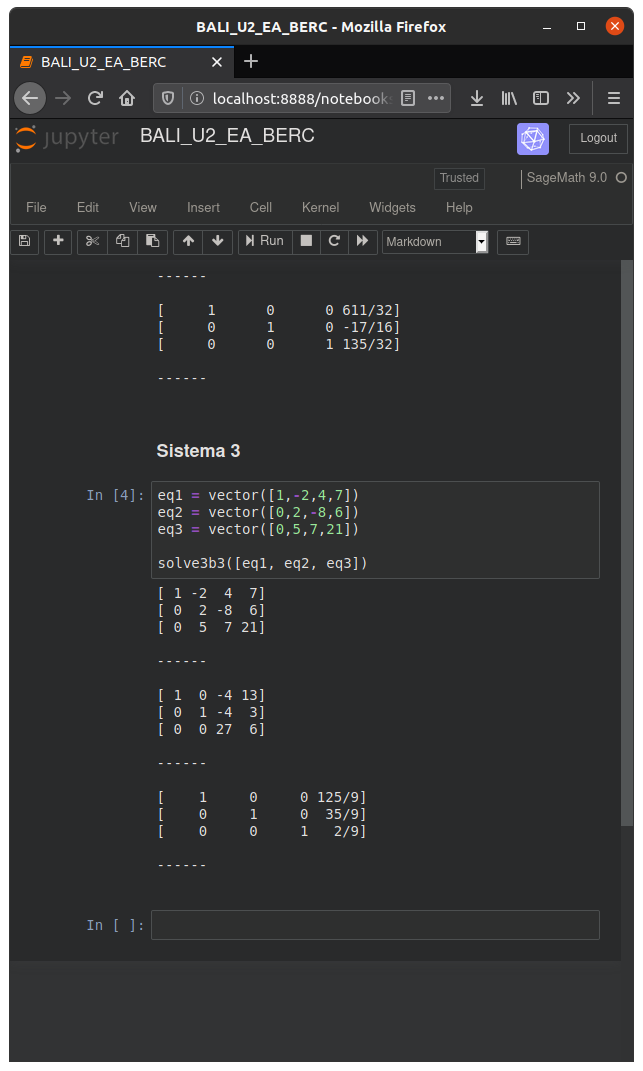
\includegraphics[width=0.32\textwidth]{BALI-U2-EA-3.png}
		\caption{Comprobaci\'on de ejercicio 1, 2 y 3}
	\end{figure}


%%%%%%%%%%%%%%%%%%%%%%%%%%%%%%%%
%%         Bibliografia        %%
%%%%%%%%%%%%%%%%%%%%%%%%%%%%%%%%%%

\newpage
\begin{thebibliography}{X}

	\bibitem{biblio} UnADM. (S/D). \emph{Primer semestre Algebra Lineal}. \today, de Universidad Abierta y a Distancia de México \textbar{} DCSBA Sitio web: \url{https://dmd.unadmexico.mx/contenidos/DCSBA/BLOQUE1/BI/01/BALI/unidad_01/descargables/BALI_U1_Contenido.pdf}
	\bibitem{github} BenchHPZ. (2020). Biotecnolog\'ia. \today, de GitHub Sitio web: \url{https://github.com/BenchHPZ/UnADM-Biotecnologia}
	
\end{thebibliography}


\end{document}